\documentclass[12pt,oneside]{book}
\usepackage[utf8]{inputenc}
\usepackage[T1]{fontenc}
\usepackage{amsmath}
\usepackage{amsfonts}
\usepackage{amssymb}
\usepackage[none]{hyphenat}
\usepackage[a4paper,width=150mm,top=23mm,bottom=22mm,bindingoffset=6mm]{geometry}
\usepackage{pdfpages}
%\usepackage{fancyhdr}
%\pagestyle{fancy}
\usepackage{graphicx}
\usepackage{csquotes}
\usepackage[titles]{tocloft}
\setlength{\cftbeforechapskip}{6pt}
\usepackage{titlesec}
\graphicspath{{images/}}
\usepackage{caption}
\usepackage{subcaption}
\usepackage{wrapfig}
\usepackage{multicol}
\usepackage{multirow}
\usepackage{mathtools}
\usepackage{longtable}
\usepackage{setspace}
\usepackage{enumitem}
\usepackage{natbib}
\bibliographystyle{abbrvnat}
\setcitestyle{authoryear,open={(},close={)}}
\usepackage[hidelinks]{hyperref} 
\usepackage[printonlyused]{acronym}
\DeclarePairedDelimiter{\norm}{\lVert}{\rVert}

\begin{document}

\frontmatter

\begin{titlepage}
	\begin{center}
		\vspace*{1cm}
		
		\LARGE
		\textbf{KWAME NKRUMAH UNIVERSITY OF SCIENCE AND TECHNOLOGY, KUMASI} \\
		COLLEGE OF SCIENCE \\
		DEPARTMENT OF MATHEMATICS
	
		\vspace{0.7in}
		
		
\includegraphics[scale=0.8]{logo}
		
		\vspace{0.7in}
		
		\textbf{APPLICATION OF MACHINE LEARNING IN PREDICTING HOSTEL PRICES: A Case Study of KNUST}
		
		\vspace{0.3in}
		
		\large
			BY \\ \vspace{0.3in}
			ANNAN JESSE \\
			BOATENG GLORIA MAAME SERWAA \\
			DENTE-QUARSHIE OBENG KWAME
		
	\end{center}
\end{titlepage}

\renewcommand{\arraystretch}{1.3}
\renewcommand{\baselinestretch}{0}

\addcontentsline{toc}{chapter}{ABSTRACT}
\chapter*{ABSTRACT}
\begin{sloppypar}
	
Machine learning, which dates back to the 1950s, aims to make accurate predictions with unseen (similar) data based on patterns discovered in existing data. In the real estate market, machine learning algorithms have been deployed in either determining house price indexes or estimating house sale prices. The latter is being studied the most by considering factors such as location, population, proximity to a nearby station, zip code, and many more. However, research on hostel price prediction is rare, if not nonexistent. To help bridge the gap, we will explore the impact of hostel features using three machine learning algorithms: multiple linear regression, ridge regression, and neural network, in predicting hostel prices. Empirical results support the potential of machine learning algorithms on the hostel market, with all $R^2 $ greater than 0.75.

\end{sloppypar}

\addcontentsline{toc}{chapter}{ACKNOWLEDGMENTS}
\chapter*{ACKNOWLEDGMENTS}
The completion of this project could not have been possible without the assistance of numerous people. Therefore, we would like to express our deep appreciation and indebtedness to our supervisor, Dr. Charles Sebil, whose insightful leadership and knowledge helped us complete this project successfully. \newline
We would also like to express our deep appreciation to Dr. Emmanuel Kofi Gavu and Ms. Deborah Dormah Kanubala for their valuable suggestions and ideas towards the completion of this project and to all the lecturers we have encountered. We thank you for allowing us to glean knowledge from you throughout our stay here. \newline
Finally, we would like to thank all our relatives, family, and friends who supported us in one way or another. Above all, we would like to thank God Almighty for always showering us with his blessings.

\tableofcontents

\addcontentsline{toc}{chapter}{LIST OF ABBREVIATIONS}
\chapter*{List of Abbreviations}
\begin{acronym}

	\acro{ml}[ML]{Machine Learning}
	\acro{mlr}[MLR]{Multiple Linear Regression}
	\acro{lr}[LR]{Lasso Regression}
	\acro{rr}[RR]{Ridge Regression}
	\acro{nn}[NN]{Neural Network}
	\acro{relu}[ReLU]{Rectified Linear Unit}
	\acro{mar}[MAR]{Missing At Random}
	\acro{mcar}[MCAR]{Missing Completely At Random}
	\acro{nmar}[NMAR]{Not Missing At Random}
	\acro{prss}[PRSS]{Penalized Residual Sum of Squares}
	\acro{mad}[MAD]{Median Absolute Deviations}
	\acro{mae}[MAE]{Mean Absolute Error}
	\acro{rmse}[RMSE]{Root Mean Squared Error}
	\acro{cos}[CoS]{College of Science}
	\acro{pha}[PHA]{Private Hostels Association}
	\acro{src}[SRC]{Students' Representative Council}
	\acro{knust}[KNUST]{Kwame Nkrumah University of Science and Technology}
		
\end{acronym}


\mainmatter

\chapter{INTRODUCTION}
% \chapter{INTRODUCTION}

\begin{sloppypar}

		\section{Background}
		Renting a hostel is undoubtedly one of the most important decisions a student makes during their entire stay on campus. The price of these hostels depends on a wide variety of factors, ranging from location to the number of beds in a room, access to the shuttle, and many more. As the population of students increases, traditional hostel price predictions based on hostel price comparisons lacking an accepted standard can no longer be employed to estimate hostel prices. Therefore, the availability of a hostel price prediction model helps fill an important information gap \citep{Calhoun2003} and boosts the hostel market efficiency. \ac{ml} is one of the cutting-edge techniques that can be utilized to identify, interpret, and analyze hugely complicated data structures and patterns \citep{Ngiam2019}.
		
		\subsection{Machine Learning Overview}
		Machine Learning \citep{Douglass2020} is the science of programming computers to learn from data. The three major types of \ac{ml} are supervised, unsupervised, and reinforcement learning. In supervised learning, the \ac{ml} is guided with desired inputs and outputs by a human operator; the algorithm learns from the data and makes predictions. A typical supervised learning task is regression. Unsupervised learning algorithms find insight in unlabeled training data and organize the data in some way to describe its structure; a typical task is clustering. Reinforcement learning \citep{Youplus2018} is a type of machine learning technique that enables an agent to learn in an interactive environment by trial and error using feedback from its actions and experiences; the commonly used algorithm is Q-learning.
		
		
		\section{Problem Statement}
		In developed countries, \ac{ml} has been implemented successfully to estimate real estate prices. However, in Ghana, the application of \ac{ml} is rare and few and far between on the topic of hostels. The lack of adequate data \citep{Owusu-Ansah2012} has made it difficult, if not impossible, to develop efficient or systematic hostel pricing policies through modeling the hostel market. As a result, hostel managers always overprice their hostel rooms. This study aims to derive valuable insight into KNUST's hostel market through analyzing a real historical dataset. It seeks useful models to illustrate how \ac{ml} algorithms can be utilized to predict hostel prices given a set of its features.
		
		
		\section{Significance}
		Our models, if accepted, could allow students or hostel managers to make better decisions. In addition, it could benefit the projection of future hostel prices and the policy-making process for the hostel market.
		
		
		\section{Limitations}
		\begin{itemize}%[leftmargin=*]
			\item This paper proves the competence of \ac{ml} algorithms in the hostel market. Although it aims to assist policymakers in projecting future hostel prices, it does not, however, explicitly forecast hostel prices.
			
			\item 70 out of 105 recommended hostels by \ac{knust}; were considered for this study.
			
			\item Although several students rent homes (homestels), this study only focused solely on the prices of private hostels around KNUST. 
		\end{itemize}	
		
		\section{Outline}
		The next parts of this paper are constructed as follows: In Chapter 2, existing literature on housing market prediction applying different \ac{ml} algorithms will be reviewed. Chapter 3 explores the dataset, explains how to transform it into cleaned data, and introduces the various supervised \ac{ml} algorithms implemented. Chapter 4 presents our empirical results and the conclusion deduced in Chapter 5.
			
\end{sloppypar}

\chapter{LITERATURE REVIEW}
% \chapter{LITERATURE REVIEW}

\begin{sloppypar}
	
	\section{Introduction}
	Previous studies on the real estate market using \ac{ml} approaches can be categorized into two groups: the trend forecasting of house price indexes and house price valuations \citep{Phan2019}. Since house prices are strongly correlated to other factors such as location, area, and population \citep{Kamal2021b}, it requires other information apart from the house price index to predict individual house prices \citep{Truong2020}.
	
	
	\section{Related Work}
	\citep{Gavu2019a}, one of the very few papers to model the residential rental housing market in Ghana, implemented the hedonic price model to estimate house prices in the Accra Metropolis, Adenta, Ga East, La Dade Kotopon, and La Nkwantanang Madina areas while exploring the existence of submarkets. \newline
	\citep{panhouse} implemented and compared the performance of Ridge, Lasso, Multiple Linear Regression, Neural Nets, and Random Forest. In their findings, neural networks proved to be the most accurate in estimating house value. \newline
	\citep{Selim2009} and \citep{Limsombunchai2004a} papers offer a comparative approach between hedonic model and artificial neural network, although, on different datasets, results show that artificial neural network performs significantly better. On the other hand, \citep{Nguyen2001} compared multiple linear regression and artificial neural networks. Empirical results show that the performance of artificial neural networks improved as the data size increased. \newline
	$ L_1 $ and $ L_2 $ regularization was implemented by \citep{Xin2018} on a housing dataset from 2006 to 2010, lasso regression ($ L_1 $) produced much better predictions; while \citep{Madhuri2019}, involved Multiple Linear, Elastic Net, Gradient Boosting, and Ada Boost regression together with $ L_1 $ and $ L_2 $ regularization for estimating house price value; with a score of approximately 0.92, Gradient Boosting proved superior. \newline
	\citep{Thamarai2020a} applied Multiple Linear Regression and Decision Tree Regression to a housing dataset. Comparatively, the performance of multiple linear regression produced better results. \newline 
	\citep{Vineeth2018} modeled a Kaggle housing dataset utilizing 19 regression algorithms to help consumers find a price for their soon-to-be house without consulting a real estate agent (broker). Cat boost was the best performing model based on RMSE, with a value of $2.604e+04 $.

\end{sloppypar}

\chapter{METHODOLOGY}
% \chapter{METHODOLOGY}

\begin{sloppypar}
	
	\section{Introduction}
	In this chapter, we explore our data, perform data preparations, and feature engineering on the dataset, then we build, compare, and evaluate three models: neural network, linear, and ridge regression.


	\section{Exploratory Data Analysis}
	Exploratory data analysis refers to the critical process of performing initial investigations on data to discover patterns, spot anomalies, test hypotheses, and check assumptions with the help of summary statistics and graphical representations \citep{Patil}. Visualizations not shown in this section are allocated in the appendix. \newline
	Figure \ref{fig:t2} shows skewed data of the target feature and \ref{fig:lnp1} shows the transformation of the target feature using a natural log, which is deemed to have a normal distribution.
	
	\begin{figure}[h!]
	\centering	
	\begin{subfigure}{0.49\textwidth}
		\centering
		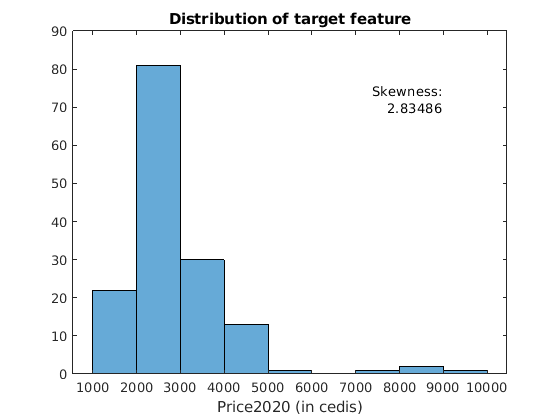
\includegraphics[width=\textwidth]{target2}
		\caption{Distribution of price2020}
		\label{fig:t2}
	\end{subfigure}
	\hfill
	\begin{subfigure}{0.49\textwidth}
		\centering
		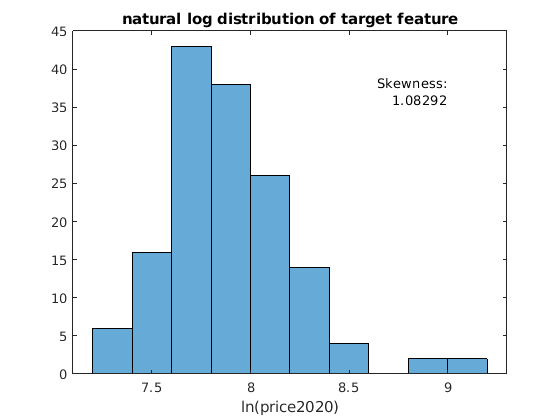
\includegraphics[width=\textwidth]{lnprice1}
		\caption{Distribution of ln(price2020)}
		\label{fig:lnp1}
	\end{subfigure}
	\caption{Histograms of target feature 1}	
	\label{fig:dist}
	\end{figure}

	
	\section{Data Preparation}
	Data preparation is the act of manipulating raw data (which may come from disparate data sources) into a form that can readily and accurately be analyzed \citep{Davidf}. In light of that, we first deal with missing data and remove inputs that behave like outliers. Next, we select important features and feature engineer the categorical features.

	\subsection{Missing Data}
	Most \ac{ml} algorithms cannot work with missing features \citep{Douglass2020}. Missing data are unobserved values that would be meaningful for analysis if observed. In other words, a missing value hides a meaningful value \citep{little1988}.
	
	\begin{table}[h!]
		\centering
		\caption{Missing Data in hostels dataset}
		\label{table:3}
		\begin{tabular}{|c|cccc|}
			\hline
			\textbf{Feature} & grade & rank & price2018 & price2019 \\ \hline
			\textbf{\%Missing} & 3\% & 3\% & 89\% & 64\% \\
			\textbf{numMissing} & 5 & 5 & 135 & 97 \\ \hline
			\textbf{numTotal} & \multicolumn{4}{|c|}{242} \\ \hline
		\end{tabular}
	\end{table}
	
	\hspace*{-0.6cm}The two types of missingness observed in our dataset are \ac{mar} and \ac{mcar}. The grade is of type \ac{mcar} since respondents chose to skip answering; hence they were fixed using the imputation method. Rank is of type \ac{mar} considering its value depends on the grade. price2018 and price2019 are of type \ac{mcar} because, in most cases, respondents were not present in their hostels during those academic years and thus discarded completely.
	
	\subsection{Outliers}
	By default, an outlier is a value that is more than three scaled \ac{mad} away from the dataset \citep{Mathworks}. Outliers can easily affect the performance of the model\citep{Parashar2021}. Hence, we use $ 99\% $ of our dataset to reduce their effect on the data (and models).
	
	\subsection{Feature Selection} 
	Feature selection is a subfield within \ac{ml} aimed at creating accurate models by excluding irrelevant features and including only relevant features \citep{Jaiantilal2013}. Features are selected based on their scores in various statistical tests (e.g., Pearson's correlation) for their correlation with the outcome variable.
	
	\subsection{Feature Engineering}
	Every \ac{ml} model is based on some mathematical concept, so we encode every categorical value into a numerical value. Features without inherent order, such as study\_room were one-hot-encoded, and features with inherent order, such as rank, were label encoded.
	Also, beds and post\_code features were deemed categorical since they contain 4 and 21 distinct responses, respectively, with no inherent order. Therefore, we one-hot-encoded the two features.
	
	\subsection{Data Splitting}
	Data splitting is the process of partitioning our available data into a train set (for training all models) and a test set (to evaluate the models). Using the cvpartition object together with the Mersenne Twister random number generator (i.e., rng (1)) in Matlab (R2021a), the cleaned dataset will be randomly partitioned, with 65\% as a training set and 35\% as a test set.
	
	
	\section{Model Selection}
	\subsection{Criteria to Measure Performance}
	The test set were evaluated using: \ac{mae}, \ac{rmse} and Coefficient of Determination ($ R^2 $)
	
	\subsubsection{Mean Absolute Error (MAE)}
	\begin{equation} \label{eqn:mae}
	MAE = \frac{1}{n}\sum_{i=1}^{n} |e_i| = \frac{1}{n}\sum_{i=1}^{n} |y_i - \hat{y}_i|
	\end{equation}
		
	\subsubsection{Root Mean Squared Error (RMSE)}
	\begin{equation} \label{eqn:rmse}
		RMSE = \sqrt{ \frac{1}{n} SSE } = \sqrt{ \frac{1}{n} \sum_{i=1}^{n} (y_i - \hat{y}_i)^2 } 
	\end{equation}
	
	\subsubsection{Coefficient of Determination ($R^2$)}
	\[SST = \sum_{i=1}^{n} (y_i - \bar{y})^2 \ \ \ \ \ \ \ SSE =  \sum_{i=1}^{n} (y_i - \hat{y})^2 \]
	\begin{equation} \label{eqn:r2}
	R^2 = 1 - \frac{SSE}{SST}
	\end{equation}
	
	\subsection{Predictive Modeling}
	\subsubsection{Linear Regression}
	Linear regression \citep{Chatterjee2013} is a linear approach to modeling the relationship between a response and one or more explanatory variables. Given a dataset $ \{x_{1i}, x_{2i}, ..., x_{pi}, y_i\} $ of $ n $ sets of observations, it is assumed that these observations satisfy a linear relationship,
	\begin{equation} \label{eqn:mlr}
	y_i = \beta_o + \beta_1 x_{1i} + \beta_2 x_{2i} + \cdots + \beta_p x_{pi} + \epsilon_i = X \beta + \epsilon
	\end{equation}
	A primary goal of regression analysis is to estimate the unknown parameters $ \beta$. The standard approach is least squares regression, where the estimates chosen to minimize are,
	\begin{equation} \label{eqn:ols}
	\norm{y - X\beta}_2^2 = \sum_{i=1}^{n} [ y_i - (\beta_o + \beta_1 x_{1i} + \cdots + \beta_p x_{pi}) ]^2
	\end{equation}
	
	\hspace*{-0.6cm}The normal equation which determines the minimizer of \ref{eqn:ols} is,
	\begin{equation}
	\hat{\beta} = (X^{T}X)^{-1}X^{T}y
	\end{equation}
	
	\subsubsection{Ridge Regression}
	\ac{rr} \citep{Shewhart2015} is a method of estimating the coefficients of \ac{mlr} models in scenarios where independent variables are highly correlated. \newline
	The theory was first introduced by Hoerl and Kennard in 1970 \citep{hoerl1970ridge}. However, \ac{rr} is a special case of Tikhonov regularization \citep{tikhonov1966stability}, in which all parameters are equally regularized. The \ac{prss} is,
		\begin{equation} \label{eqn:prss}
		\norm{y - X\beta}_2^2 + \lambda \norm{\beta}_2^2
		\end{equation}
		\ac{rr} estimate coefficients in \ref{eqn:prss} using
		\begin{equation}
		\hat{\beta}_{ridge} = (X^{T} X + \lambda I)^{-1} X^{T} y
		\end{equation}
		Where $ \lambda $ is the shrinkage parameter and $ I $, an identity matrix.
	
	\subsubsection{Neural Network}
	\ac{nn} is an interconnected group of nodes inspired by a simplification of neurons in the brain. The network learns by adjusting weights to reduce the prediction error\citep{han2011data}. Initially, all weights and biases are randomly allocated. The algorithm then runs iteratively, and each iteration comprises two steps: forward feeding and backpropagation \citep{Phan2019}.

		\begin{itemize}%[leftmargin=*]
			\item In the forward feeding phase, the output for the computation unit, $ a_i^{k+1} $ is the result of applying a transfer function, $ \sigma $ to the summation of all signals from each connection, $ a_i^k $ times the value of the connection weight, $ W_{ji} $ between node $ a_i^{k+1} $ and connection $ a_i^{k} $ \citep{coakley2000artificial}. The prediction of the output layer is then compared to the observed outcome to derive the learning rate and errors \citep{Phan2019}.
			\begin{eqnarray}
			z_j = \sum_j (W_{ji}^k a_i^k) \\
			a_i^{k+1} = \sigma (z_j)
			\end{eqnarray}
			\begin{equation*}
			where \ \ \ \sigma = ReLU(x) = max(0,x)
			\end{equation*}
			
			where $a$ is the activation of unit $ i $ in layer $ k $, $W_j$ is the weight of unit $ i $ in layer $ k $  and $\sigma$ is the transfer function, \ac{relu}.
			
			\item In backpropagation, given the learning rate and errors, the network recalculates the weights and bias in hidden layers and makes appropriate changes to reduce prediction errors \citep{Phan2019}.
		\end{itemize}
	
\end{sloppypar}

\chapter{DATA COLLECTION, ANALYSIS AND RESULTS}
% \chapter{DATA COLLECTION, ANALYSIS AND RESULTS}

\begin{sloppypar}
	
	\section{Original Dataset}
	For this study, data obtained were through interviews with student residents in the hostels.
	The dataset is a cleaned dataset from 495 responses from 70 distinct hostels (Table \ref{table:2}).
	Since most hostels can be located in Ayeduase and Kotei, 38 and 20 hostels were selected from Ayeduase and Kotei, respectively, and 6 each from Bomso and Kentinkrono.

		\begin{longtable}{p{3cm}p{3cm}p{7cm}}
			\caption{Features Description} 
			\label{table:1} \\
			\hline
			\textbf{Name} & \textbf{Type} & \textbf{Description} \\ \hline
			location & categorical & general location of hostel \\ %\hline
			grade & numerical & average of students' evaluation \\ %\hline
			rank & categorical & overall quality of hostel \\ %\hline
			beds & numerical & beds in a room \\ %\hline
			study room & categorical & hostel's study room \\ %\hline
			tv room & categorical & hostel's tv room \\ %\hline
			security & categorical & security personnel or post \\ %\hline
			food joint & categorical & food joint within 5 minutes walk \\ %\hline
			external power & categorical & another source of power \\ %\hline
			ac & categorical & air conditioner in a room \\ %\hline
			proximity & numerical & distance to \ac{cos} \\ %\hline
			post code & categorical & post code of hostel \\ %\hline
			latitude & numerical & hostel's latitude \\ %\hline
			longitude & numerical & hostel's longitude \\ %\hline
			price2018 & numerical & price of room for 2018/19 in cedis \\ %\hline
			price2019 & numerical & price of room for 2019/20 in cedis \\ %\hline
			price2020 & numerical & price of room for 2020/21 in cedis (target feature) \\ \hline
		\end{longtable}
	
	
	\section{Results}
	First, we check the assumption of \ac{mlr} model. Figure \ref{fig:var} shows no notable patterns in our residuals and a negligible correlation; hence, equality of variance and independence of observation assumptions are met. Figure \ref{fig:norm} shows a plot with data points close to the normal line; a t-test on the residuals produced a p-value of $ >> 0.05 $; as a result, the normality assumption can be accepted. Since all assumptions are met, the \ac{mlr} model qualifies as a candidate model for our dataset.
	\vspace*{0.5cm}
	
	\begin{figure}[h]
		\centering
		\begin{subfigure}[h]{0.47\textwidth}
			\centering
			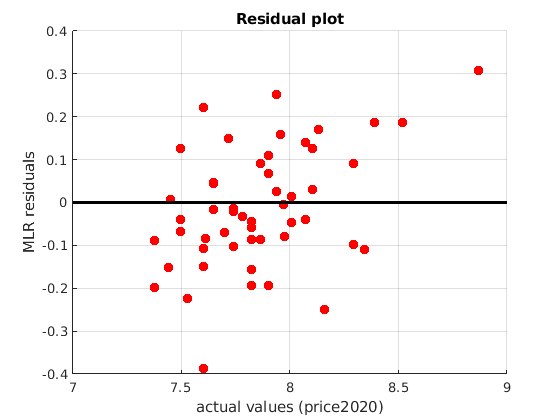
\includegraphics[width=\textwidth]{lmres}
			\caption{Equality of Variance}
			\label{fig:var}
		\end{subfigure}
		\hfill
		\begin{subfigure}[h]{0.47\textwidth}
			\centering
			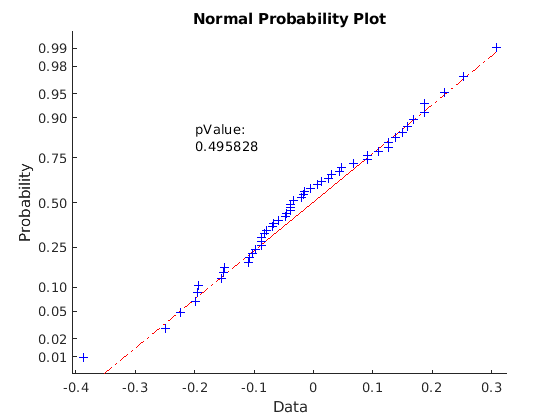
\includegraphics[width=\textwidth]{lmprob}
			\caption{Normality of Residuals}
			\label{fig:norm}
		\end{subfigure}
		\caption{Analysis of Residuals}
		\label{fig:allerr}
	\end{figure}
	
	\hspace*{-0.6cm}The evaluation metrics given by equations \ref{eqn:mae}, \ref{eqn:rmse} and \ref{eqn:r2} of both train and test sets are presented in Table \ref{table:metric}
	
	\begin{table}[h!]
		\centering
		\caption{Evaluation Metrics of Train and Test sets}
		\label{table:metric}
		\begin{tabular}{|c|p{1.5cm}p{1.5cm}c|p{1.5cm}p{1.5cm}c|}
			\hline
			\multirow{2}{*}{MODELS} & \multicolumn{3}{|c|}{TRAIN SET} & \multicolumn{3}{|c|}{TEST SET} \\ \cline{2-7}
			& MAE & RMSE & $R^2$ & MAE & RMSE & $R^2$ \\ \hline
			\ac{mlr} & 0.1069 & 0.1337 & 0.7968 & 0.1114 & 0.1382 & 0.79 \\
			\ac{rr} & 0.1142 & 0.1406 & 0.7753 & 0.1116 & 0.1443 & 0.7711 \\
			\ac{nn} & 0.1069 & 0.1337 & 0.7968 & 0.1125 & 0.1398 & 0.7852 \\ \hline
		\end{tabular}
	\end{table} 
	
	\hspace*{-0.6cm}From Table \ref{table:metric}, all three models performed well, with all coefficients of determination of the test set close to 1. However, the \ac{rr} which was implemented to improve the fit in \ac{mlr} utilizing its embedded feature selection properties with lambda of 0.0103, produced an $ R^2 $ lesser than the \ac{mlr} model. Moreover, the \ac{mlr} generalized well on the test set with an $ R^2 $ of 0.79; this could be as a result of no or negligible over-fitting and/or issues of collinearity. \newline
	The \ac{nn} modeled the relationship between predictors and target features with two layers - a hidden layer with 10 nodes and an output layer with 1 node. The model, as noted by \citep{Phan2019}, works like a "black box," and we do not know the relationship between the predictors and the price prediction. Even so, the model performed exactly as \ac{mlr} model on the train set. However, on the test set, there was a reduction in all three evaluation metrics (Figure \ref{table:metric}).
	\newpage  
	\hspace*{-0.6cm}Using the same models developed by our machine learning algorithms by learning from the entire dataset, we will explore the existence of submarkets \citep{maclennan1996economic} in the AYEDUASE and KOTEI areas using the table below.
	
	\begin{table}[h!]
		\centering
		\caption{Evaluation Metrics of submarkets}
		\label{table:metric2}
		\begin{tabular}{|c|p{1.5cm}p{1.5cm}c|p{1.5cm}p{1.5cm}c|}
			\hline
			\multicolumn{7}{|c|}{AYEDUASE} \\
			\hline \hline
			\multirow{2}{*}{MODELS} & \multicolumn{3}{|c|}{TRAIN SET} & \multicolumn{3}{|c|}{TEST SET} \\ \cline{2-7}
			& MAE & RMSE & $R^2$ & MAE & RMSE & $R^2$ \\ \hline
			\ac{mlr} & 0.1175 & 0.1487 & 0.6544 & 0.1253 & 0.1488 & 0.7786 \\
			\ac{rr} & 0.1194 & 0.15 & 0.6486 & 0.1327 & 0.1596 & 0.7451 \\
			\ac{nn} & 0.1175 & 0.1487 & 0.6544 & 0.1253 & 0.1488 & 0.7786 \\ \hline \hline
			\multicolumn{7}{|c|}{KOTEI} \\
			\hline \hline
			\multirow{2}{*}{MODELS} & \multicolumn{3}{|c|}{TRAIN SET} & \multicolumn{3}{|c|}{TEST SET} \\ \cline{2-7}
			& MAE & RMSE & $R^2$ & MAE & RMSE & $R^2$ \\ \hline
			\ac{mlr} & 0.0913 & 0.1131 & 0.8686 & 0.1003 & 0.1188 & 0.8126 \\
			\ac{rr} & 0.0899 & 0.1192 & 0.8541 & 0.0854 & 0.1011 & 0.8642 \\
			\ac{nn} & 0.0913 & 0.1131 & 0.8686 & 0.1004 & 0.1188 & 0.8126 \\ \hline
		\end{tabular}
	\end{table}
	
	\hspace*{-0.6cm}In Table \ref{table:metric2} above, \ac{mlr} and \ac{nn} models produced similar results. However, the low number of observations may be a possible explanation for the poor performance of all models on the train set in the "AYEDUASE" submarket.
	

\end{sloppypar}

\chapter{CONCLUSION AND RECOMMENDATIONS}
% \chapter{CONCLUSION AND RECOMMENDATION}

\begin{sloppypar}
		
	\section{Conclusion}
	In summary, this study is an exploratory attempt to use three machine learning algorithms to estimate hostel prices and then compare their performances after carefully preparing, transforming, and clearing the dataset. In this study, our models are trained with some hostel features and 2019/20 prices utilizing \ac{mlr}, \ac{rr} and \ac{nn}. We have demonstrated the predictive power of machine learning algorithms on the hostel market, as evaluated by the performance metrics. \newline
	Given our dataset used in this paper, our main conclusion is that \ac{mlr} and \ac{nn} can generate comparably accurate hostel price estimations with lower prediction errors, compared with the \ac{rr} results. Based on these estimates, we hope hostel managers, \ac{src} and \ac{pha} will incorporate this approach in estimating hostel prices or developing new policies that govern the hostel market. \newline
	Furthermore, results from Table \ref{table:metric2} prove the existence of a hostel submarket in the AYEDUASE and KOTEI areas, with all $ R^2 $ greater than 0.8 on the test sets.
		
		
	\section{Recommendation}
	First, the non-linear relationship between proximity and hostel price, which is mostly the main reason students rent hostels, should be explored using other algorithms such as random forest and decision trees. \newline
	Moreover, from our dataset, post\_code contains 21 unique area codes. Further investigations into the hostel market should consider reducing the complexity of the feature by employing an unsupervised machine learning algorithm for cluster analysis to reduce the number of features during training. \newline
	Finally, this paper considered only the 2019/20 academic year information for the hostels. The time effect of the hostel price, which could potentially impact the estimated results, was removed due to the sparsity of such data. Therefore, we suggest that different data collection styles should be employed.
		
\end{sloppypar}



\backmatter

\addcontentsline{toc}{chapter}{REFERENCES}
\renewcommand{\bibname}{REFERENCES}
\bibliography{ref}

\pagestyle{plain}

\addcontentsline{toc}{chapter}{APPENDIX A: Additional Informative Figures and Tables}
\chapter*{ {APPENDIX A:} \\ {Additional Informative Figures} \\ {and Tables} }
\appendix

\pagestyle{plain}

\begin{figure}[h!]
	\centering	
	\begin{subfigure}{0.49\linewidth}
		\centering
		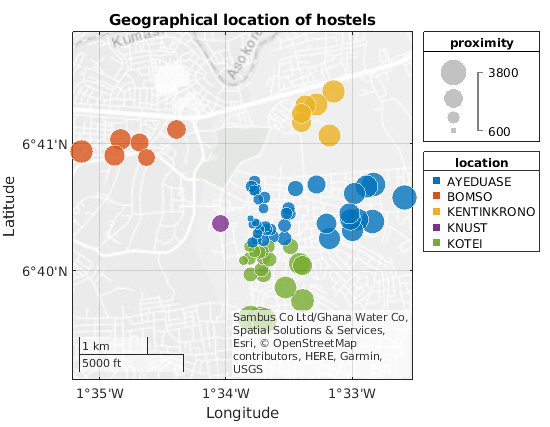
\includegraphics[width=\textwidth]{geo1.png}
		\caption{Geographical location of hostels}
		\label{fig:geo1}
	\end{subfigure}
	\hfill
	\begin{subfigure}{0.49\linewidth}
		\centering
		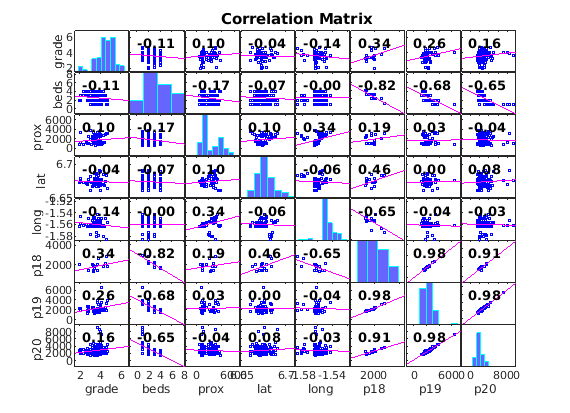
\includegraphics[width=\textwidth]{corr.png}
		\caption{Correlation matrix}
		\label{fig:corr}
	\end{subfigure}
\end{figure}


\begin{figure}[h!]
	\centering
	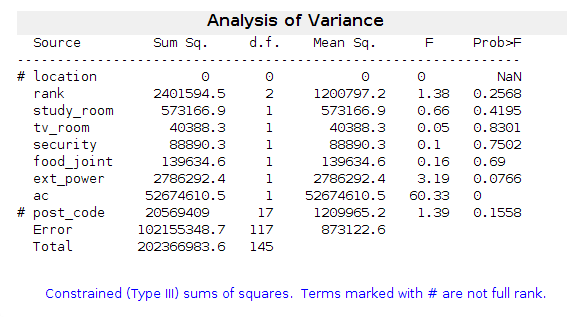
\includegraphics[scale=0.65]{anova.png}
	\caption{ANOVA table}
	\label{fig:anova}
\end{figure}

\newpage

\begin{longtable}{p{6.5cm}p{6.5cm}}
	\caption{List of hostels and their location}
	\label{table:2} \\
	\hline
	\textbf{hostel} & \textbf{location} \\
	\hline
	ADOM - BI & AYEDUASE \\
	AFRIM &	AYEDUASE \\
	AMANDAH & AYEDUASE \\
	AMEN MAIN & AYEDUASE \\
	AMERICAN HOUSE & AYEDUASE \\
	ANAROSA & KOTEI \\
	ANGLICAN & KENTINKRONO \\
	B. O. EXECUTIVE & AYEDUASE \\
	BANIVILLAS & KENTINKRONO \\
	BEACON & AYEDUASE \\
	BLUE ARK & BOMSO \\
	BY HIS GRACE & AYEDUASE \\
	CANAM & KOTEI \\
	CASA MARIA & AYEDUASE \\
	CELIA ROYAL & KOTEI \\
	CHRISTIAN IPS & BOMSO \\
	CRYSTAL ROSE & KENTINKRONO \\
	DAKENS INTERNATIONAL & AYEDUASE \\
	DELISA MAIN & AYEDUASE \\
	DEVALYPAH & KOTEI \\
	ENIN & AYEDUASE \\
	FNF & AYEDUASE \\
	F – PLAZA & AYEDUASE \\
	FLINT & KOTEI \\
	FOSUA HOMES & AYEDUASE \\ 
	FRANCO & KOTEI \\
	FRONTLINE INN & AYEDUASE \\
	GAZA & KENTINKRONO \\
	GEORGIA & KENTINKRONO \\
	HALLOWED & KOTEI \\
	HAPPY FAMILY & AYEDUASE \\
	HIGH ACHIEVERS & AYEDUASE \\
	HYDES & AYEDUASE \\ 
	JALEX & AYEDUASE \\
	JOHANNES & KOTEI \\
	K GEE & AYEDUASE \\
	KWAKYEWAA & KOTEI \\
	LONG ISLAND & KOTEI \\
	MANCHESTER & KOTEI \\
	MASS & KOTEI \\
	MILLENNIUM LIGHT & AYEDUASE \\
	MORNING STAR PALACE & BOMSO \\
	NANA ADOMAH & AYEDUASE \\
	NEVADA & AYEDUASE \\
	NO WEAPON & KOTEI \\
	NYAME MIREKU & AYEDUASE \\
	NYANTAKYI & AYEDUASE \\
	ORANGE & KOTEI \\
	P 3 HOSTEL & AYEDUASE \\
	PINAMANG & AYEDUASE \\
	PRESTIGE & KOTEI \\
	PROVIDENCE & KOTEI \\
	RISING STAR (NYBERG) & AYEDUASE \\
	RISING SUN & AYEDUASE \\
	ROYAL GATE & BOMSO \\ 
	SHALOM KIBBUTZ & AYEDUASE \\
	SHEPHERDSVILLE & AYEDUASE \\
	SOMPA & KOTEI \\
	SPLENDOR & AYEDUASE \\
	STANDARD & BOMSO \\
	SUN CITY & KENTINKRONO \\
	THE BEST & KOTEI \\
	THY KINGDOM COME & AYEDUASE \\
	THY WILL BE DONE & KOTEI \\
	ULTIMATE & BOMSO \\
	VICTORY TOWERS & AYEDUASE \\
	WAGYINGO & AYEDUASE \\
	WEST END & AYEDUASE \\
	WHITE HOUSE & AYEDUASE \\
	WHITPAM A & KOTEI \\ \hline
\end{longtable}

\end{document}